\section{Einleitung}

Die erste Arbeit, die heute dem Bereich der künstlichen Intelligenz (KI) zugeordnet wird, wurde 1943 von McCulloch und Pitts geleistet \cite{McCulloch1943}.
Sie ließen sich in ihrer Arbeit von Neuronen im Gehirn inspirieren und erstellten erste mathematische Formulierungen welche später großen Einfluss in der Entwicklung neuraler Netze hatten.
Die Neuronen werden dabei als Schalter gesehen, dessen Aktivierung durch andere Neuronen beeinflusst wird.
Auf diese weise lassen sich komplexe Systeme erstellen, welche in der Lage sind unterschiedliche Aufgaben zu lösen.
Der Begriff der künstlichen Intelligenz selbst wurde 1956 von McCarthy geprägt, als er einen zweimonatigen Workshop in Dartmouth \cite{McCarthy1955} organisierte.

Nach den anfänglich großen Erwartungen an die künstliche Intelligenz, ohne die versprochenen Ergebnisse zu liefern, erhielt das Gebiet weniger Aufmerksamkeit.
Ein berühmtes Zitat von Herbert Simon aus dem Jahr 1957 ist:
\begin{quotation}
    Es ist nicht mein Ziel, Sie zu überraschen oder zu schockieren - aber ich kann am einfachsten zusammenfassen, dass es jetzt in der Welt Maschinen gibt, die denken, die lernen und die schaffen. Darüber hinaus wird ihre Fähigkeit, diese Dinge zu tun, rasch zunehmen, bis - in einer sichtbaren Zukunft - die Bandbreite der Probleme, die sie bewältigen können, mit der Bandbreite, auf die der menschliche Verstand angewandt wurde, übereinstimmen wird.
\end{quotation}

Entgegen dieser Übertreibungen wurden im Laufe der Jahrzehnte allerdings dennoch Fortschritte erzielt.
Nach einer weiteren Periode hoher Investitionen in den 1980er Jahren, ohne die ehrgeizigen Ziele zu erreichen, setzte der so genannte "KI-Winter" ein, der sich durch mangelndes akademisches und wirtschaftliches Interesse und mangelnde Finanzierung bemerkbar machte.

In jüngster Zeit jedoch finden Forschung und Anwendung dieser Techniken wieder mehr Aufmerksamkeit.
Dies ist auf einige in der heutigen Zeit vorherrschende Faktoren zurückzuführen.
Zum einen ist es die schiere Menge an Rechenleistung, die moderne Computern haben können.
Selbst Heimcomputer sind heute in der Lage, Modelle von bemerkenswerter Komplexität zu trainieren.

Des Weiteren erleichtert die Menge an Daten, die durch das Internet zur Verfügung steht, das Training der KIs für verschiedene Aufgaben.
Um ein Modell für eine bestimmte Aufgabe zu trainieren, werden geeignete Daten benötigt, um korrekte Vorhersagen über nie gesehene Daten zu treffen (Generalisierung).
Da Daten in großer Menge zur Verfügung stehen, gibt es entsprechend mehrere Datenbanken für Forschung, Training und Evaluation.
Eine Liste von Datenbanken kann unter \aka{https://en.wikipedia.org/wiki/List_of_datasets_for_machine-learning_research} eingesehen werden.

Deshalb wird der künstlichen Intelligenz in der Forschung immer mehr Aufmerksamkeit geschenkt, und immer mehr praktische Bereiche betrachten diese Technik als Lösung für verschiedenste Problemstellungen.
Ob der jüngste Enthusiasmus nur übertriebene Erwartungen sind, oder ob die "letzte Erfindung der Menschheit" \cite{Good1965} nahe ist, bleibt abzuwarten.

Der Begriff künstliche Intelligenz wird verwendet, um maschinelle Vorgänge zu beschreiben, die Aufgaben ausführen, die sonst charakteristisch für die menschliche Intelligenz sind.
Diese Arbeit soll sich vor Allem mit einem Teilgebiet der künstlichen Intelligenz befassen, dem so genannten "deep learning".
Dieser Zusammenhang ist in Abbildung \ref{fig:ai_ml_dl} dargestellt.

\begin{figure}
    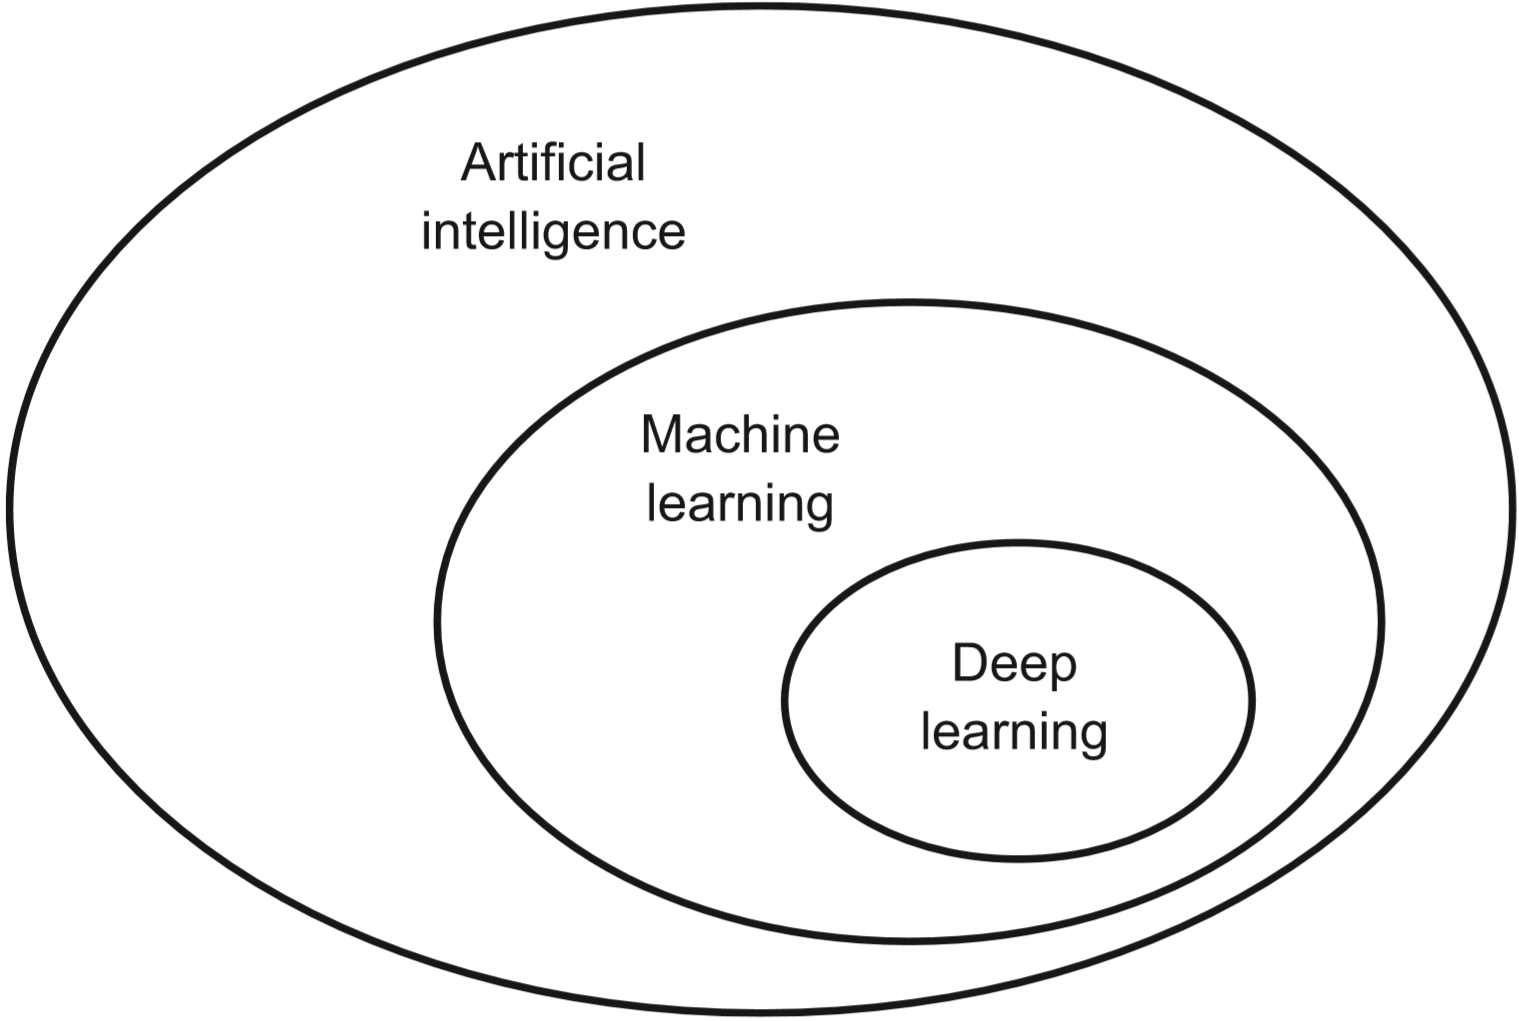
\includegraphics[width=0.5\textwidth]{images/ai_ml_dl.png}
    \caption[KI, ML und DL]{Künstliche Intelligenz, Maschinelles Lernen und Deep Learning \cite[p.4]{Chollet2017}}
    \label{fig:ai_ml_dl}
\end{figure}

In diesem Projekt möchte ich maschinelles Lernen in das Gebiet der Kinematik für zweidimensionales Skizzieren und der Prototypentwicklung mit \name{deepmech} vorstellen.
Die erste für dieses Projekt implementierte Lösung nimmt Bilder als Input und gibt den jeweiligen Typ handgeschriebener mechanischer Symbole aus.
Die mit dem vorgestellten Ansatz erstellten Modelle sind klein und meist unabhängig von der genutzten Programmiersprache, was durch die Verwendung der populären Keras \cite{Chollet}-Bibliothek auf TensorFlow \cite{Google2019} ermöglicht wird.

Einfache Demonstrationen werden mit JavaScript durchgeführt, um eine Verbindung zu einem aufstrebenden Bereich der Kinematik mit Hilfe von Web-Technologien wie \name{mec2} \cite{Goessner2019} und \name{mecEdit} \cite{Uhlig2019} herzustellen.
Für das Training des aktuellen Modells wird die Python-Implementierung von TensorFlow verwendet, da durch die bessere Ausnutzung der GPU mit CUDA \cite{nvidia2019} als Backend ein schnelleres Training der Keras-Modelle möglich ist.
Dank der Konvertierbarkeit der Modellbeschreibungen zur Nutzung in unterschiedlichen Programmiersprachen ermöglicht dies nahtlose Übergänge zwischen verschiedenen Ansätzen.

Bevor gezeigt wird, wie deepmech entwickelt wurde, sollen die Grundlagen des maschinellen Lernens behandelt werden, wobei einige einfache Beispiele als Einführung gezeigt werden und dabei die in dieser Arbeit verwendete allgemeine Terminologie eingeführt wird.
In Kapitel 3 werden die Konzepte durch die Einführung neuronaler Netze erweitert, die der Schlüssel zur Umsetzung der Funktionsweise des maschinellen Lernens in praktische Modelle sind.
Ein weiteres Thema, das behandelt werden muss, ist die Datengenerierung. Daten sind ein wichtiger Teil des Trainings statistischer Modelle, daher wird die Datenerzeugung und -augmentierung in Kapitel 4 behandelt.
Daraufhin wird das erste funktionierende Modell gezeigt.
Alle Hauptkomponenten des Prozesses werden detailliert untersucht, um ein besseres Verständnis für jede Funktion zu erhalten.
Im 6. Kapitel geht es um die Optimierung des Modells, um die Genauigkeit zu verbessern und die Größe des Modells, das in zukünftigen Anwendungen geladen wird, zu minimieren.
Abschließend wird eine Schlussfolgerung erläutert, in der die Ergebnisse evaluiert werden.
